\documentclass[tikz, border=10pt]{standalone}

\usetikzlibrary{positioning,shapes,arrows,calc}


\begin{document}

%\nodeDistA=10mm
\newdimen\nodeDistB
\nodeDistB=20mm

\tikzset{
    position/.style args={#1:#2 from #3}{
        at=(#3.#1), anchor=#1+180, shift=(#1:#2)
    }
}

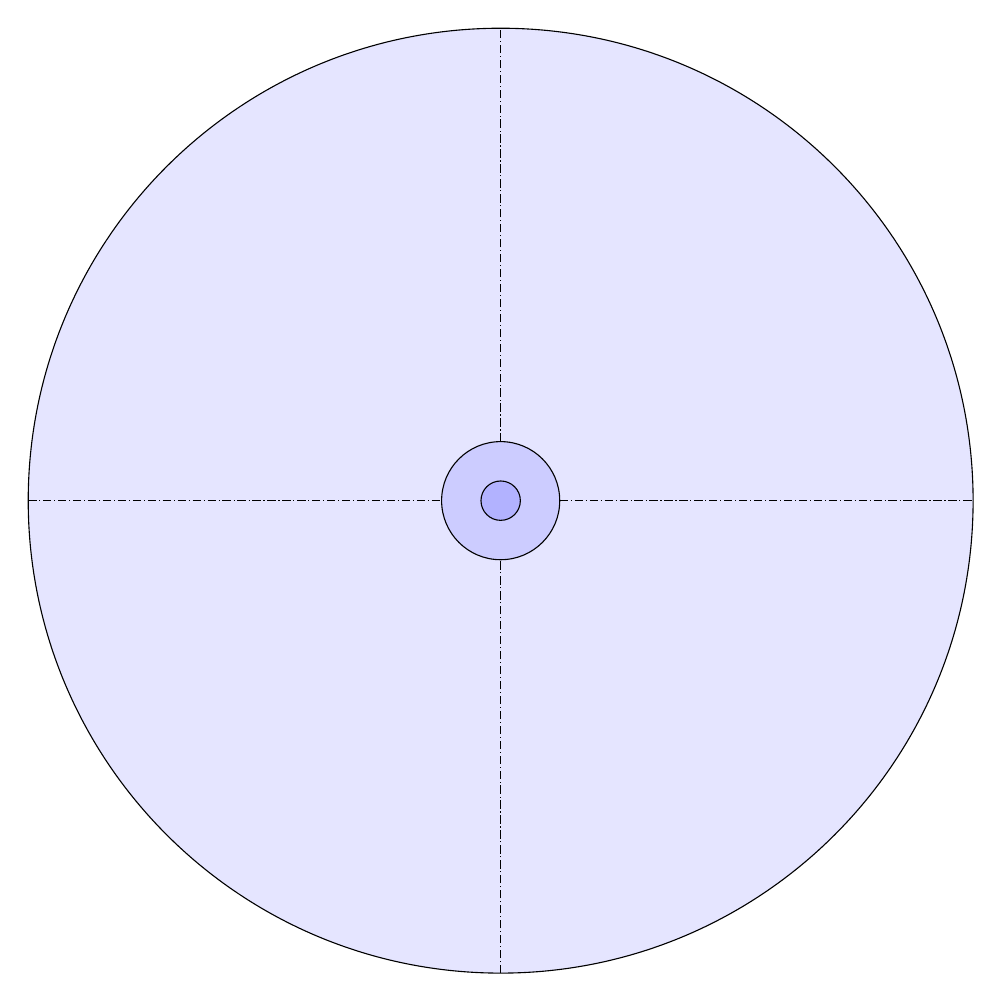
\begin{tikzpicture}
%\fontfamily{hvmath}{\fontsize{15}{15}\selectfont
%\tikzset{every node}==[font=\sffamily]
  [
    circle type 1/.style={draw=none,align=center, font=\scriptsize},
  ]
  
  \coordinate (c1) at (0,0);
  \coordinate (c2) at (6,0);
  \coordinate (c3) at (0,-6);
  \coordinate (c4) at (-6,0);
  \coordinate (c5) at (0,6);
  \coordinate (tu) at (2.95, -2.5);
  \coordinate (um1) at ($(tu) - (0,1)$);
  \coordinate (um2) at ($(tu) + (1,0)$);
  
  \newlength{\smallercircle}



  \foreach \i / \j [count=\ino] in {6/'',  0.75/fgdsfg, 0.25/fsgsdgf}
    {
     \pgfmathsetmacro{\colmixer}{mod(10*\ino,100)}%
     \path [draw, fill=blue!\colmixer] (c1) ++(0,-\i) arc (-90:270:\i);
    
    
    }
  \draw[densely dashdotted] (c4) -- ($(c1) - (0.75,0)$); 
  \draw[densely dashdotted] ($(c1) +  (0.75,0)$) -- (c2); 
  \draw[densely dashdotted] (c3) -- ($(c1) - (0,0.75)$); 
  \draw[densely dashdotted] ($(c1) + (0,0.75)$)  -- (c5); 
  
  

 
 
  %\draw (-8,-8) grid (10,10);
 

\end{tikzpicture}
\end{document}
